\documentclass[12pt,a4paper]{article}
\usepackage[utf8]{inputenc}
\usepackage[english]{babel}
\usepackage{booktabs}
\usepackage{amsmath}
\usepackage{geometry}
\usepackage{tikz}
\uset_tikz_library{automata, positioning, arrows.meta, shapes.geometric, circuits.logic.US}

\geometry{margin=2.5cm}

\title{Digital Technology: Finite State Machines \& PLDs}
\date{May 2026}

\begin{document}

\maketitle

\section{Part 1: Finite State Machines (FSM)}

\subsection{What are Finite State Machines?}
A Finite State Machine (FSM) is a mathematical model of computation. It is an abstract machine that can be in exactly one of a finite number of \textbf{states} at any given time. The FSM can change from one state to another in response to some inputs; the change from one state to another is called a \textbf{transition}.

\subsection{Description and Basic Elements}
State machines are described using \textbf{State Chart Diagrams}. The basic elements are:
\begin{itemize}
    \item \textbf{States (Circles):} Represent the conditions of the system.
    \item \textbf{Transitions (Arrows):} Represent the movement between states.
    \item \textbf{Inputs (Labels on Arrows):} The conditions that trigger a transition.
    \item \textbf{Outputs:} The signals produced by the machine (inside states for Moore, on transitions for Mealy).
\end{itemize}

\subsection{Moore vs. Mealy Machines}
\begin{itemize}
    \item \textbf{Moore Machine:} The output depends \textbf{only} on the current state.
    \item \textbf{Mealy Machine:} The output depends on the current state \textbf{and} the current input.
\end{itemize}

\subsection{Example: Pedestrian Traffic Light (Moore Machine)}
This machine controls a traffic light that stays green until a pedestrian presses a button ($X=1$).

\begin{figure}[h]
\centering
\begin{tikzpicture}[->, >=Stealth, node distance=5cm,
    every node/.style={
        circle,
        draw,
        minimum size=2.5cm,
        inner sep=0pt,
        align=center,
        line width=1.5pt,
        font=\small
    }]

    \node[fill=green!30, draw=green!60!black] (S0) {$S_0$ \\ \textbf{GREEN} \\ $Y=001$};
    \node[fill=yellow!40, draw=yellow!60!black] (S1) [right of=S0] {$S_1$ \\ \textbf{YELLOW} \\ $Y=010$};
    \node[fill=red!30, draw=red!60!black] (S3) [below of=S1] {$S_3$ \\ \textbf{RED} \\ $Y=100$};
    \node[fill=orange!40, draw=orange!60!black] (S2) [below of=S0] {$S_2$ \\ \textbf{RED-YELLOW} \\ $Y=110$};

    \path[line width=1.2pt]
        (S0) edge [loop left] node {$X=0$} (S0)
        (S0) edge node [above] {$X=1$} (S1)
        (S1) edge node [right] {Always} (S3)
        (S3) edge [loop right] node {$X=1$} (S3)
        (S3) edge node [below] {$X=0$} (S2)
        (S2) edge node [left] {Always} (S0);
\end{tikzpicture}
\caption{State Chart Diagram for the Moore Traffic Light.}
\end{figure}

\subsection{Implementation Tables}
\subsubsection{Transient Functions (Next State Logic)}
\begin{table}[h]
\centering
\begin{tabular}{ccc}
\toprule
Current State & Input ($X$) & Next State \\
\midrule
$S_0$ & 0 & $S_0$ \\
$S_0$ & 1 & $S_1$ \\
$S_1$ & X & $S_3$ \\
$S_3$ & 1 & $S_3$ \\
$S_3$ & 0 & $S_2$ \\
$S_2$ & X & $S_0$ \\
\bottomrule
\end{tabular}
\end{table}

\subsubsection{Output Functions}
\begin{table}[h]
\centering
\begin{tabular}{ccc}
\toprule
State & Bits ($y_2 y_1 y_0$) & Light \\
\midrule
$S_0$ & 001 & Green \\
$S_1$ & 010 & Yellow \\
$S_2$ & 110 & Red + Yellow \\
$S_3$ & 100 & Red \\
\bottomrule
\end{tabular}
\end{table}

\newpage
\section{Part 2: Programmable Logic Devices (PLDs)}

\subsection{SPLD, CPLD, and FPGA Definitions}
\begin{itemize}
    \item \textbf{SPLD (Simple PLD):} Smallest devices (PAL, PLA, GAL). Consist of an AND-plane and an OR-plane.
    \item \textbf{CPLD (Complex PLD):} Multiple SPLD blocks connected by a central switching matrix. Non-volatile (stays programmed without power).
    \item \textbf{FPGA (Field Programmable Gate Array):} A huge grid of logic blocks (CLBs) with distributed routing. Volatile (needs to be loaded at startup).
\end{itemize}

\subsection{PLD Schematic (AND-Plane)}
\begin{figure}[h]
\centering
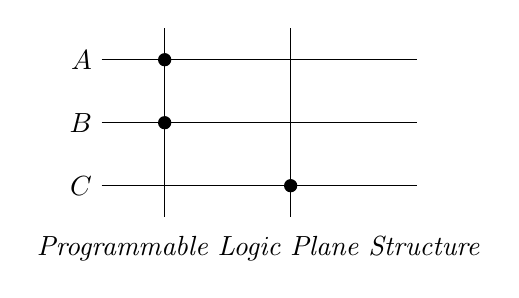
\begin{tikzpicture}[scale=0.8]
    \draw (0,3) node[left] {$A$} -- (5,3);
    \draw (0,2) node[left] {$B$} -- (5,2);
    \draw (0,1) node[left] {$C$} -- (5,1);
    \draw (1,3.5) -- (1,0.5);
    \draw (3,3.5) -- (3,0.5);
    \fill (1,3) circle (3pt);
    \fill (1,2) circle (3pt);
    \fill (3,1) circle (3pt);
    \node at (2.5, 0) {\textit{Programmable Logic Plane Structure}};
\end{tikzpicture}
\end{figure}

\subsection{Comparison Table}
\begin{table}[h]
\centering
\begin{tabular}{@{}lll@{}}
\toprule
\textbf{Feature} & \textbf{CPLD} & \textbf{FPGA} \\ \midrule
Architecture & Central Matrix & Distributed Grid (Sea of Gates) \\
Capacity & Lower & Much Higher \\
Volatility & Non-volatile (Flash) & Volatile (SRAM) \\
Timing & Predictable & Routing dependent \\
\bottomrule
\end{tabular}
\end{table}

\end{document}
